\section{Actividad 2}

\subsection*{Un transmisor con modulación de amplitud tiene como entrada una señal $m(t)=A_m\cos(2\pi f t)$ con $A_m=3$ V y $f_m=600$ Hz. 
Si la portadora posee una amplitud de 10 V y una frecuencia de 1 kHz.}  

\subsection*{a)  Calcular de manera analítica la señal de salida del modulador en tiempo y en frecuencia, graficando además los resultados. Suponer un 90\% de porcentaje de modulación. ¿Es posible realizar una detección de envolvente sobre la señal s(t)? o ¿ se requiere una detección coherente?}

En este caso la modulación es de tipo AM (DSB con portadora). La señal portadora modulada de salida se expresa como:

    \[
        s(t) = A_c \left[ 1 + k_a A_m \cos(2\pi f_m t)\right]\cos(2\pi f_c t)
    \]

donde:  

\(A_c\) es la amplitud de la portadora 

\(A_m\) es la amplitud del mensaje

 \(f_c\) es la frecuencia de la portadora
 
 \(f_m\) es la frecuencia de la señal moduladora
 
 \(k_a\) es el la sensibilidad de amplitud del modulador

 \(\mu=k_a A_m\) es el indice de modulación

Al reemplazar los valores dados por el enunciado se obtiene:

    \[
        s(t) = 10\left[1+0.9\cos(2\pi \cdot 600t)\right]\cos(2\pi \cdot 1000t)
    \]
    

Aplicando la propiedad trigonométrica del producto de cosenos:

    \[
        \cos\alpha \cos\beta = \tfrac{1}{2}\left[\cos(\alpha+\beta)+\cos(\alpha-\beta)\right],
    \]

La expresión resultante se desarrolla como:

    \[
        s(t) = A_c\ \cos(2\pi f_c t) \;+\; \frac{A_c \ \mu}{2}\Big[ \cos\big(2\pi(f_c+f_m)t\big) + \cos\big(2\pi(f_c-f_m)t\big) \Big]
    \]


Reemplazando los valores numéricos en la expresión anterior:

    \[
        s(t) = 10\cos(2\pi \cdot 1000 t) \;+\; 4.5 \cos(2\pi \cdot 1600 t) \;+\; 4.5 \cos(2\pi \cdot 400 t)
    \]


\textbf{El desarrollo en frecuencia es el siguiente:}  

La Transformada de Fourier de \(s(t)\) está formada por tres deltas centradas en las frecuencias indicadas:

    \[
        S(f) = \tfrac{A_c}{2}\big[\delta(f-f_c)+\delta(f+f_c)\big] \;+\; 
        \tfrac{A_c \ \mu}{4}\big[\delta(f-(f_c+f_m))+\delta(f+(f_c+f_m))
    \]

    \[
        \;+\;
        \delta(f-(f_c-f_m))+\delta(f+(f_c-f_m))\big]
    \]
Reemplazando por valores numéricos:

    \[
        S(f) = \tfrac{10}{2}\big[\delta(f-1000)+\delta(f+1000)\big] \;+\; 
        \tfrac{9}{4}\big[\delta(f-1600) +\delta(f+1600)
    \]
    \[
        \;+\;
        \delta(f-400)+\delta(f+400)\big]
    \]

Para que la envolvente de la señal s(t) pueda ser detectada la frecuencia de la onda portadora debe cumplir que \(f_c \gg W\). En este caso no se cumple por lo que es necesario un detector coherente para que sea posible.

En la Fig.\ref{fig:actividad_2a} se muestra tanto la señal en el tiempo como su espectro de la señal modulada s(t).

    \begin{figure}[H]
        \centering
        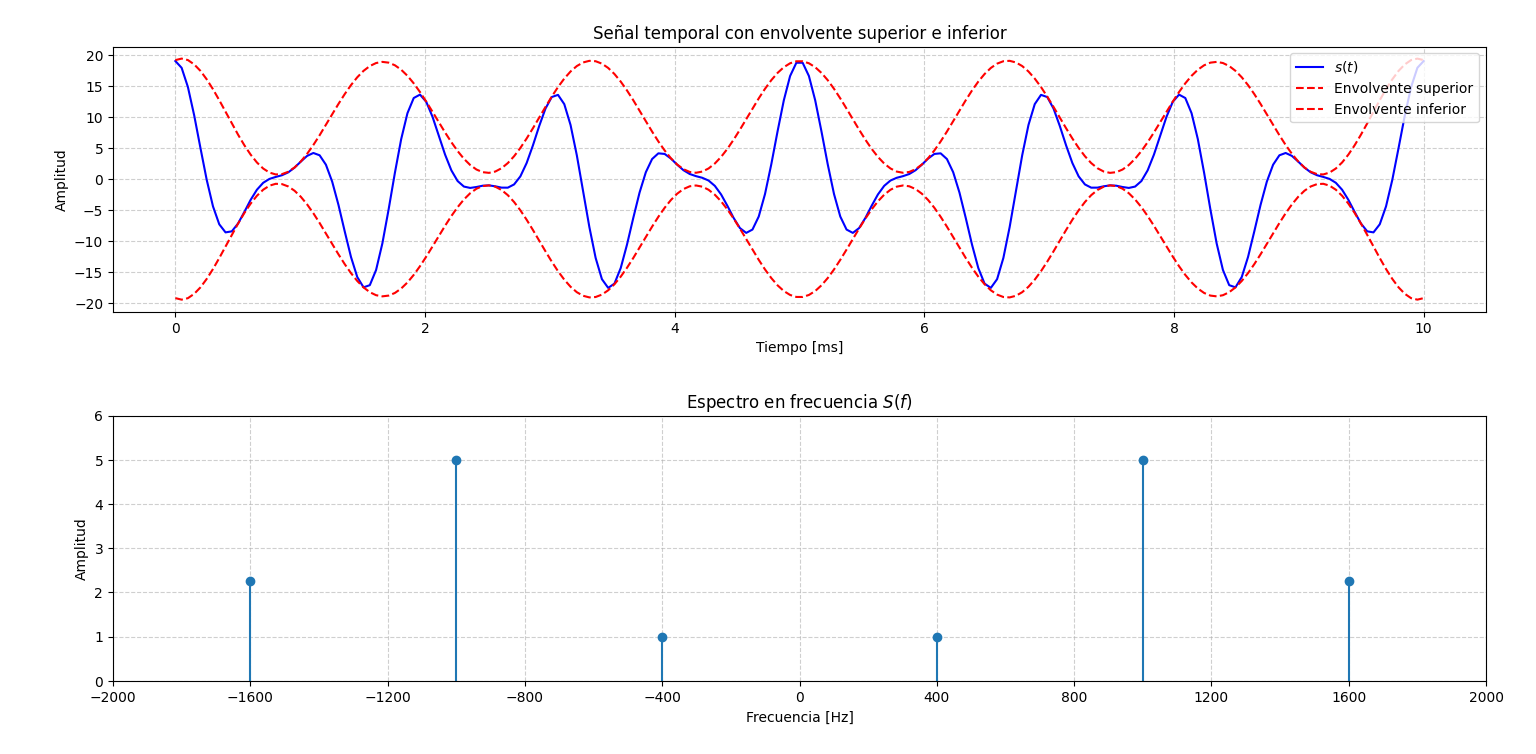
\includegraphics[width=0.9\linewidth]{imagenes/Parte_1/Actividad_2/actividad_2a.png}
        \caption{Señal modulada.}
        \label{fig:actividad_2a}
    \end{figure}

    
\subsection*{b) Modificar la frecuencia de portadora a $f_c=10f_m$ y graficar $s(t)$ para modulaciones 90\% 60\%, 20\% y 110\%. ¿Es posible detección de envolvente en todos los casos? } 

 Expresión analítica para un 90\% de $s(t)$ y $f_c=10 f_m$: 

    \[
        s(t) = 10\left[1+0.9\cos(2\pi \cdot 600t)\right]\cos(2\pi \cdot 6000t)
    \]


 Expresión analítica para un 60\% de $s(t)$ y $f_c=10 f_m$: 

    \[
        s(t) = 10\left[1+0.6\cos(2\pi \cdot 600t)\right]\cos(2\pi \cdot 6000t)
    \]


 Expresión analítica para un 20\% de $s(t)$ y $f_c=10 f_m$: 

    \[
        s(t) = 10\left[1+0.2\cos(2\pi \cdot 600t)\right]\cos(2\pi \cdot 6000t)
    \]

Expresión analítica para un 110\% de $s(t)$ y $f_c=10 f_m$: 

    \[
    s(t) = 10\left[1+1.1\cos(2\pi \cdot 600t)\right]\cos(2\pi \cdot 6000t)
    \]

En la Fig.\ref{fig:actividad_2b} se muestra las gráficas en el dominio del tiempo de la señal $s(t)$ para los distintos factores de modulación $\mu$.

    \begin{figure}[h!]
        \centering
        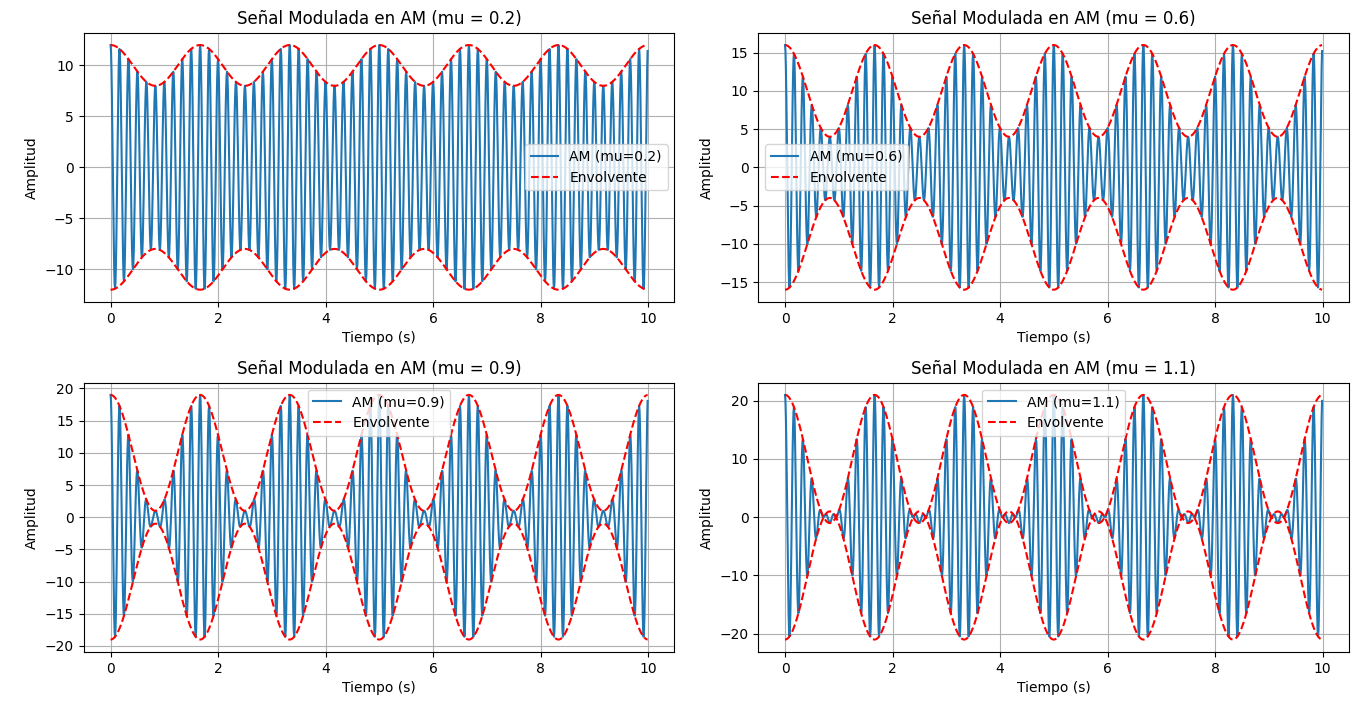
\includegraphics[width=1\textwidth]{imagenes/Parte_1/Actividad_2/actividad_2b.png}
        \caption{Gráfica de $s(t)$ para distintas $\mu$ .}
        \label{fig:actividad_2b}
    \end{figure}

Es posible la detección de envolvente en todos los casos excepto en el porcentaje de 110\% de modulación, ya que cuando la sensibilidad de amplitud $k_a$ del modulador es lo suficientemente grande como para hacer que $|k_a\,m(t)| > 1$ en algún instante de tiempo $t$, la onda portadora se convierte en \textit{sobremodulada}, resultando en una inversión de fase de la onda portadora cuando el factor $(1 + k_a\,m(t))$ cruza por cero. Entonces, la onda modulada exhibe una \textit{distorsión de envolvente}.

Por lo tanto, para evitar la sobremodulación, se debe mantener una relación uno a uno entre la envolvente de la onda AM y la onda modulante, para todos los valores del tiempo.

    

